\section{Standard Energy Meters}\label{standard-energy-meters}

Meters provide one way for EnergyPlus to report energy use in a form that is pallatable to the users. The primary implemented method for output gives very fine detail (down to the variable level) for results from EnergyPlus. However, to get the required energy use, there may be several variables that need to be polled and accumulated. The meter implementation for EnergyPlus accomplishes this reporting.

\begin{figure}[hbtp] % fig 24
\centering
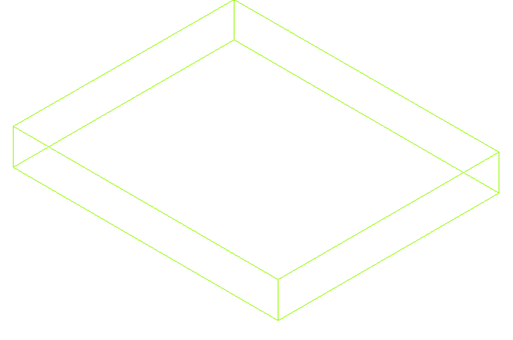
\includegraphics[width=0.9\textwidth, height=0.9\textheight, keepaspectratio=true]{media/image024.jpg}
\caption{Illustration of Energy Metering \protect \label{fig:illustration-of-energy-metering}}
\end{figure}

Meters can be used to typify energy use by type and by component. The diagrams and tables illustrate how the meters have been incorporated into EnergyPlus.

As shown in the figure above, energy use for the facility is grouped according to fuel type (see Table~\ref{table:table-of-metered-fuel-types}. Table of Metered Fuel Types), by meter type (see Table~\ref{table:overall-meter-types}. Overall Meter Types) and by end use category type (see Table~\ref{table:end-use-category-types}. End Use Category Types).

% table 7
\begin{longtable}[c]{@{}l@{}}
\caption{Overall Meter Types \label{table:overall-meter-types}} \tabularnewline
\toprule 
Meters \tabularnewline
\midrule
\endfirsthead

\caption[]{Overall Meter Types} \tabularnewline
\toprule 
Meters \tabularnewline
\midrule
\endhead

Facility \tabularnewline
Building \tabularnewline
Zone \tabularnewline
System \tabularnewline
Plant \tabularnewline
\bottomrule
\end{longtable}

Both the fuel types and enduse types are set within the program by the developers. Current Fuel types are shown in the table below. There is also a special category called ``EnergyTranser''.

% table 8
\begin{longtable}[c]{@{}l@{}}
\caption{Table of Metered Fuel Types \label{table:table-of-metered-fuel-types}} \tabularnewline
\toprule 
Utility/Fuel Types \tabularnewline
\midrule
\endfirsthead

\caption[]{Table of Metered Fuel Types} \tabularnewline
\toprule 
Utility/Fuel Types \tabularnewline
\midrule
\endhead

Electricity \tabularnewline
Gas \tabularnewline
Gasoline \tabularnewline
Diesel \tabularnewline
Coal \tabularnewline
FuelOil\#1 \tabularnewline
FuelOil\#2 \tabularnewline
Propane \tabularnewline
Water \tabularnewline
Steam \tabularnewline
DistrictCooling \tabularnewline
DistrictHeatingWater \tabularnewline
DistrictHeatingSteam \tabularnewline
\bottomrule
\end{longtable}

\begin{longtable}[c]{@{}l@{}}
\toprule 
AdditionalTypes \tabularnewline
\midrule
\endfirsthead

\toprule 
AdditionalTypes \tabularnewline
\midrule
\endhead

HeatingCoils \tabularnewline
CoolingCoils \tabularnewline
Chillers \tabularnewline
Boilers \tabularnewline
Baseboard \tabularnewline
HeatRecoveryForCooling \tabularnewline
HeatRecoveryForHeating \tabularnewline
\bottomrule
\end{longtable}

The end use types are shown in the following table:

% table 9
\begin{longtable}[c]{@{}l@{}}
\caption{End Use Category Types \label{table:end-use-category-types}} \tabularnewline
\toprule 
End Use Types \tabularnewline
\midrule
\endfirsthead

\caption[]{End Use Category Types} \tabularnewline
\toprule 
End Use Types \tabularnewline
\midrule
\endhead

InteriorLights \tabularnewline
ExteriorLights \tabularnewline
InteriorEquipment \tabularnewline
ExteriorEquipment \tabularnewline
Fans \tabularnewline
Pumps \tabularnewline
Heating \tabularnewline
Cooling \tabularnewline
HeatRejection \tabularnewline
Humidifier \tabularnewline
HeatRecovery \tabularnewline
DHW \tabularnewline
Cogeneration \tabularnewline
Refrigeration \tabularnewline
Miscellaneous \tabularnewline
\bottomrule
\end{longtable}

Additional End Use Types Only Used for EnergyTransfer:

\begin{longtable}[c]{@{}l@{}}
\toprule 
AdditionalTypes \tabularnewline
\midrule
\endfirsthead

\toprule 
AdditionalTypes \tabularnewline
\midrule
\endhead

HeatingCoils \tabularnewline
CoolingCoils \tabularnewline
Chillers \tabularnewline
Boilers \tabularnewline
Baseboard \tabularnewline
HeatRecoveryForCooling \tabularnewline
HeatRecoveryForHeating \tabularnewline
\bottomrule
\end{longtable}
